\section{4. Architecture}

In every diagram an arrow points the way the data flows and is labelled with
what flows and the protocol. A two-way arrow says which way each part goes.

\subsection{4.1 Context diagram (C4 Level 1)}

\begin{figure}[H]
\centering
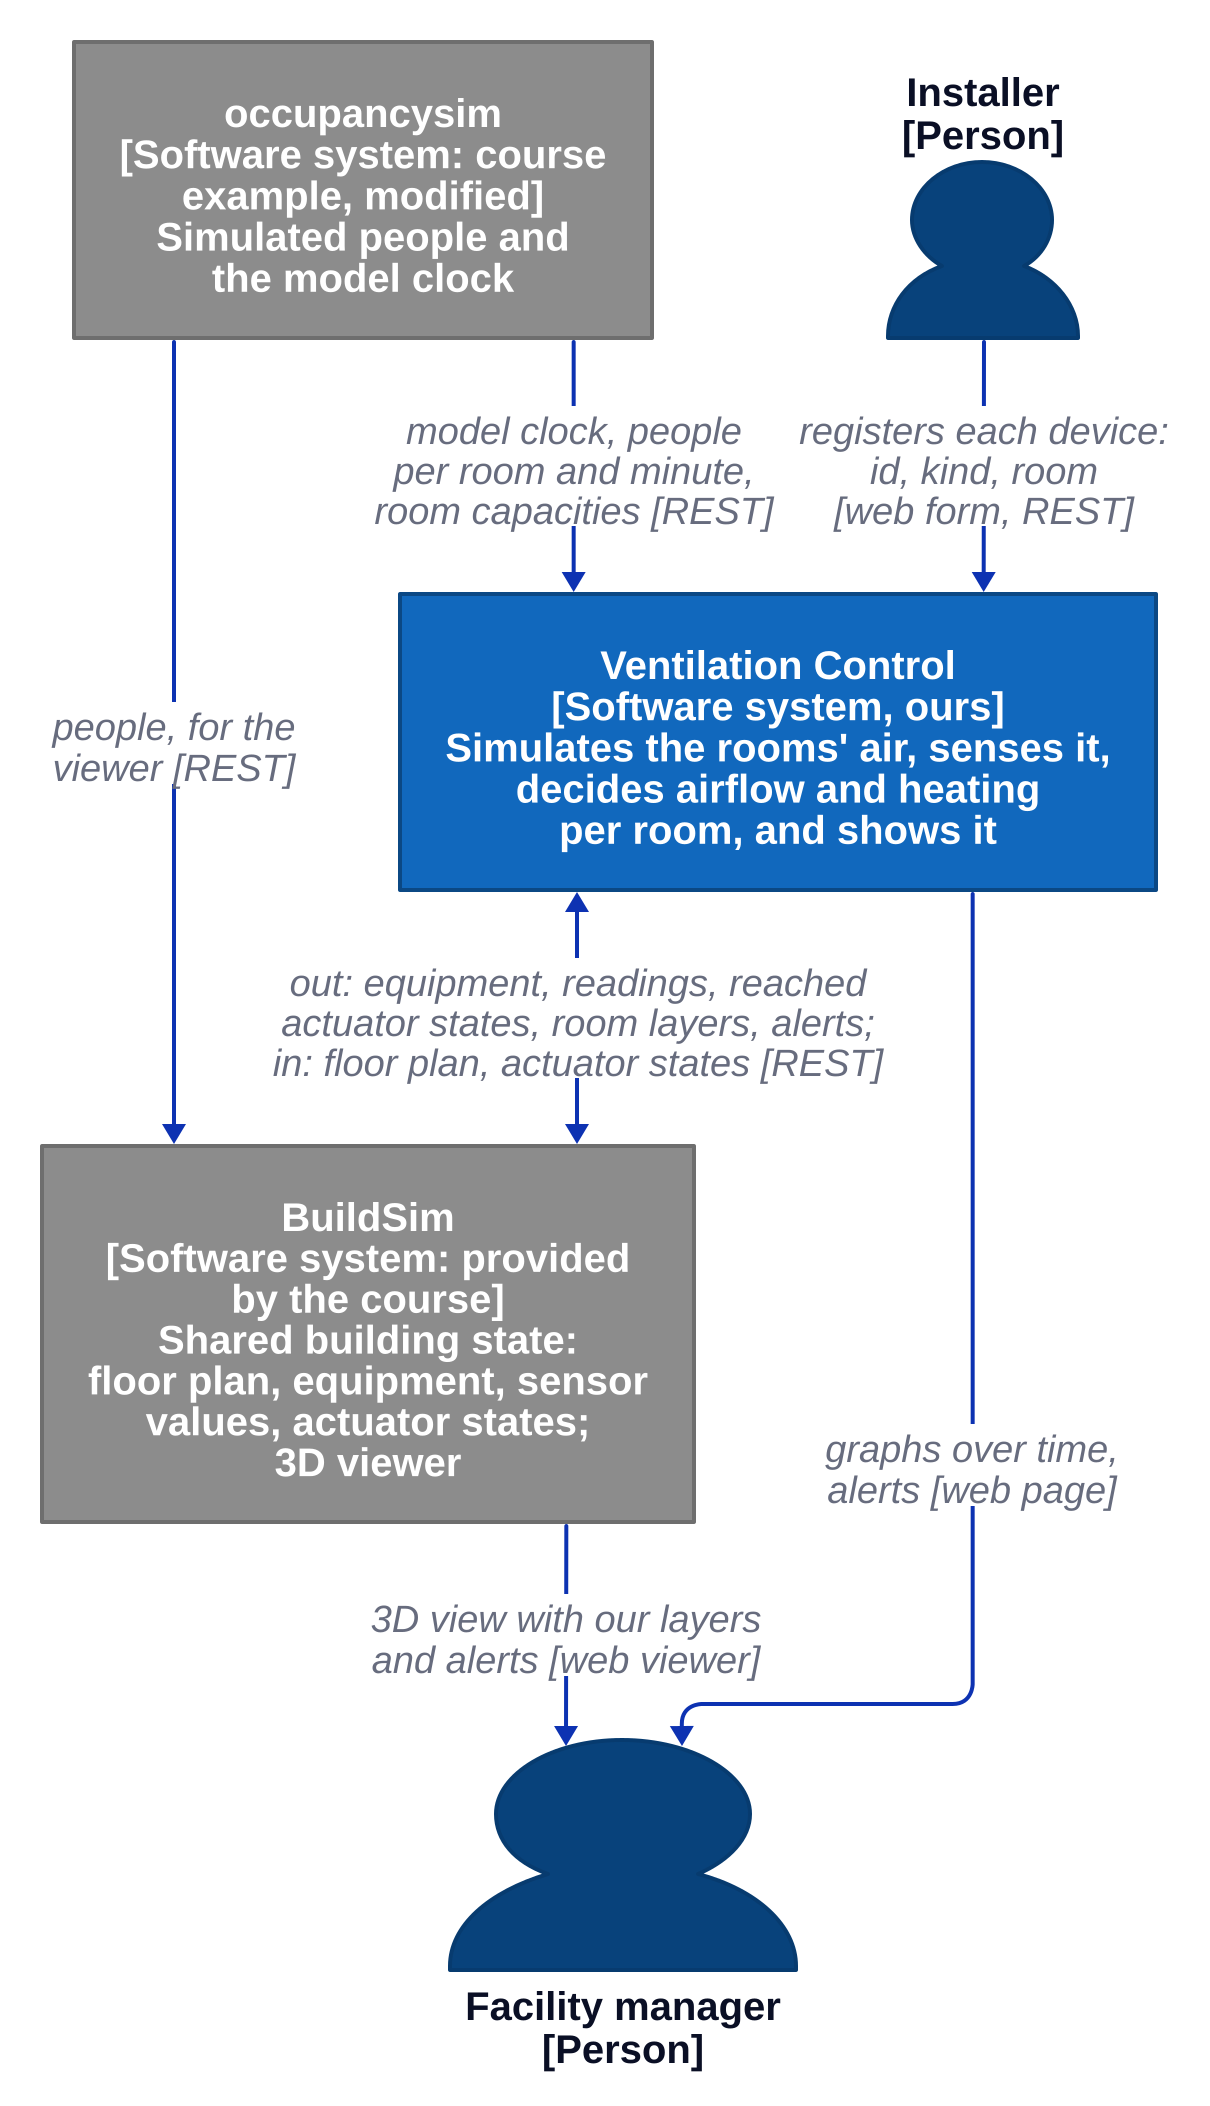
\includegraphics[width=0.52\linewidth]{figures/context.png}
\caption{System context. Our system is the blue box; the two grey systems come
from the course.}
\label{fig:context}
\end{figure}

\textbf{The boundary.} Everything we built is inside \emph{Ventilation
Control}, including the simulated room physics and the simulated devices. In a
real building those two would be the building itself and bought hardware; here
they are ours to write, and they are kept apart from the control side by the
truth boundary described in Section 4.2. \emph{BuildSim} is provided
infrastructure that we do not modify. \emph{occupancysim} is a course example
that we use as the source of people and of the model clock; we changed it in
two places (Section 6) and list the changes in \code{external/README.md}.

\textbf{The interactions.} The installer tells the system which device is in
which room. occupancysim supplies the clock and who is in each room at each
minute. Our system writes equipment, sensor readings, reached actuator states,
room layers and alerts to BuildSim, and reads the floor plan and the actuator
states back. The facility manager looks at the result in two places: BuildSim's
3D viewer, which shows the building now, and our own page, which shows it over
time.

\subsection{4.2 Container diagram (C4 Level 2)}

The container level is drawn as two views, because every link in one picture
is too dense to read on a page. Figure~\ref{fig:container} is the control loop
and the data path. Figure~\ref{fig:container-support} is commissioning and the
dashboard. Together they show every container and every link; the table after
them maps each box to its compose service and code folder.

\begin{figure}[H]
\centering
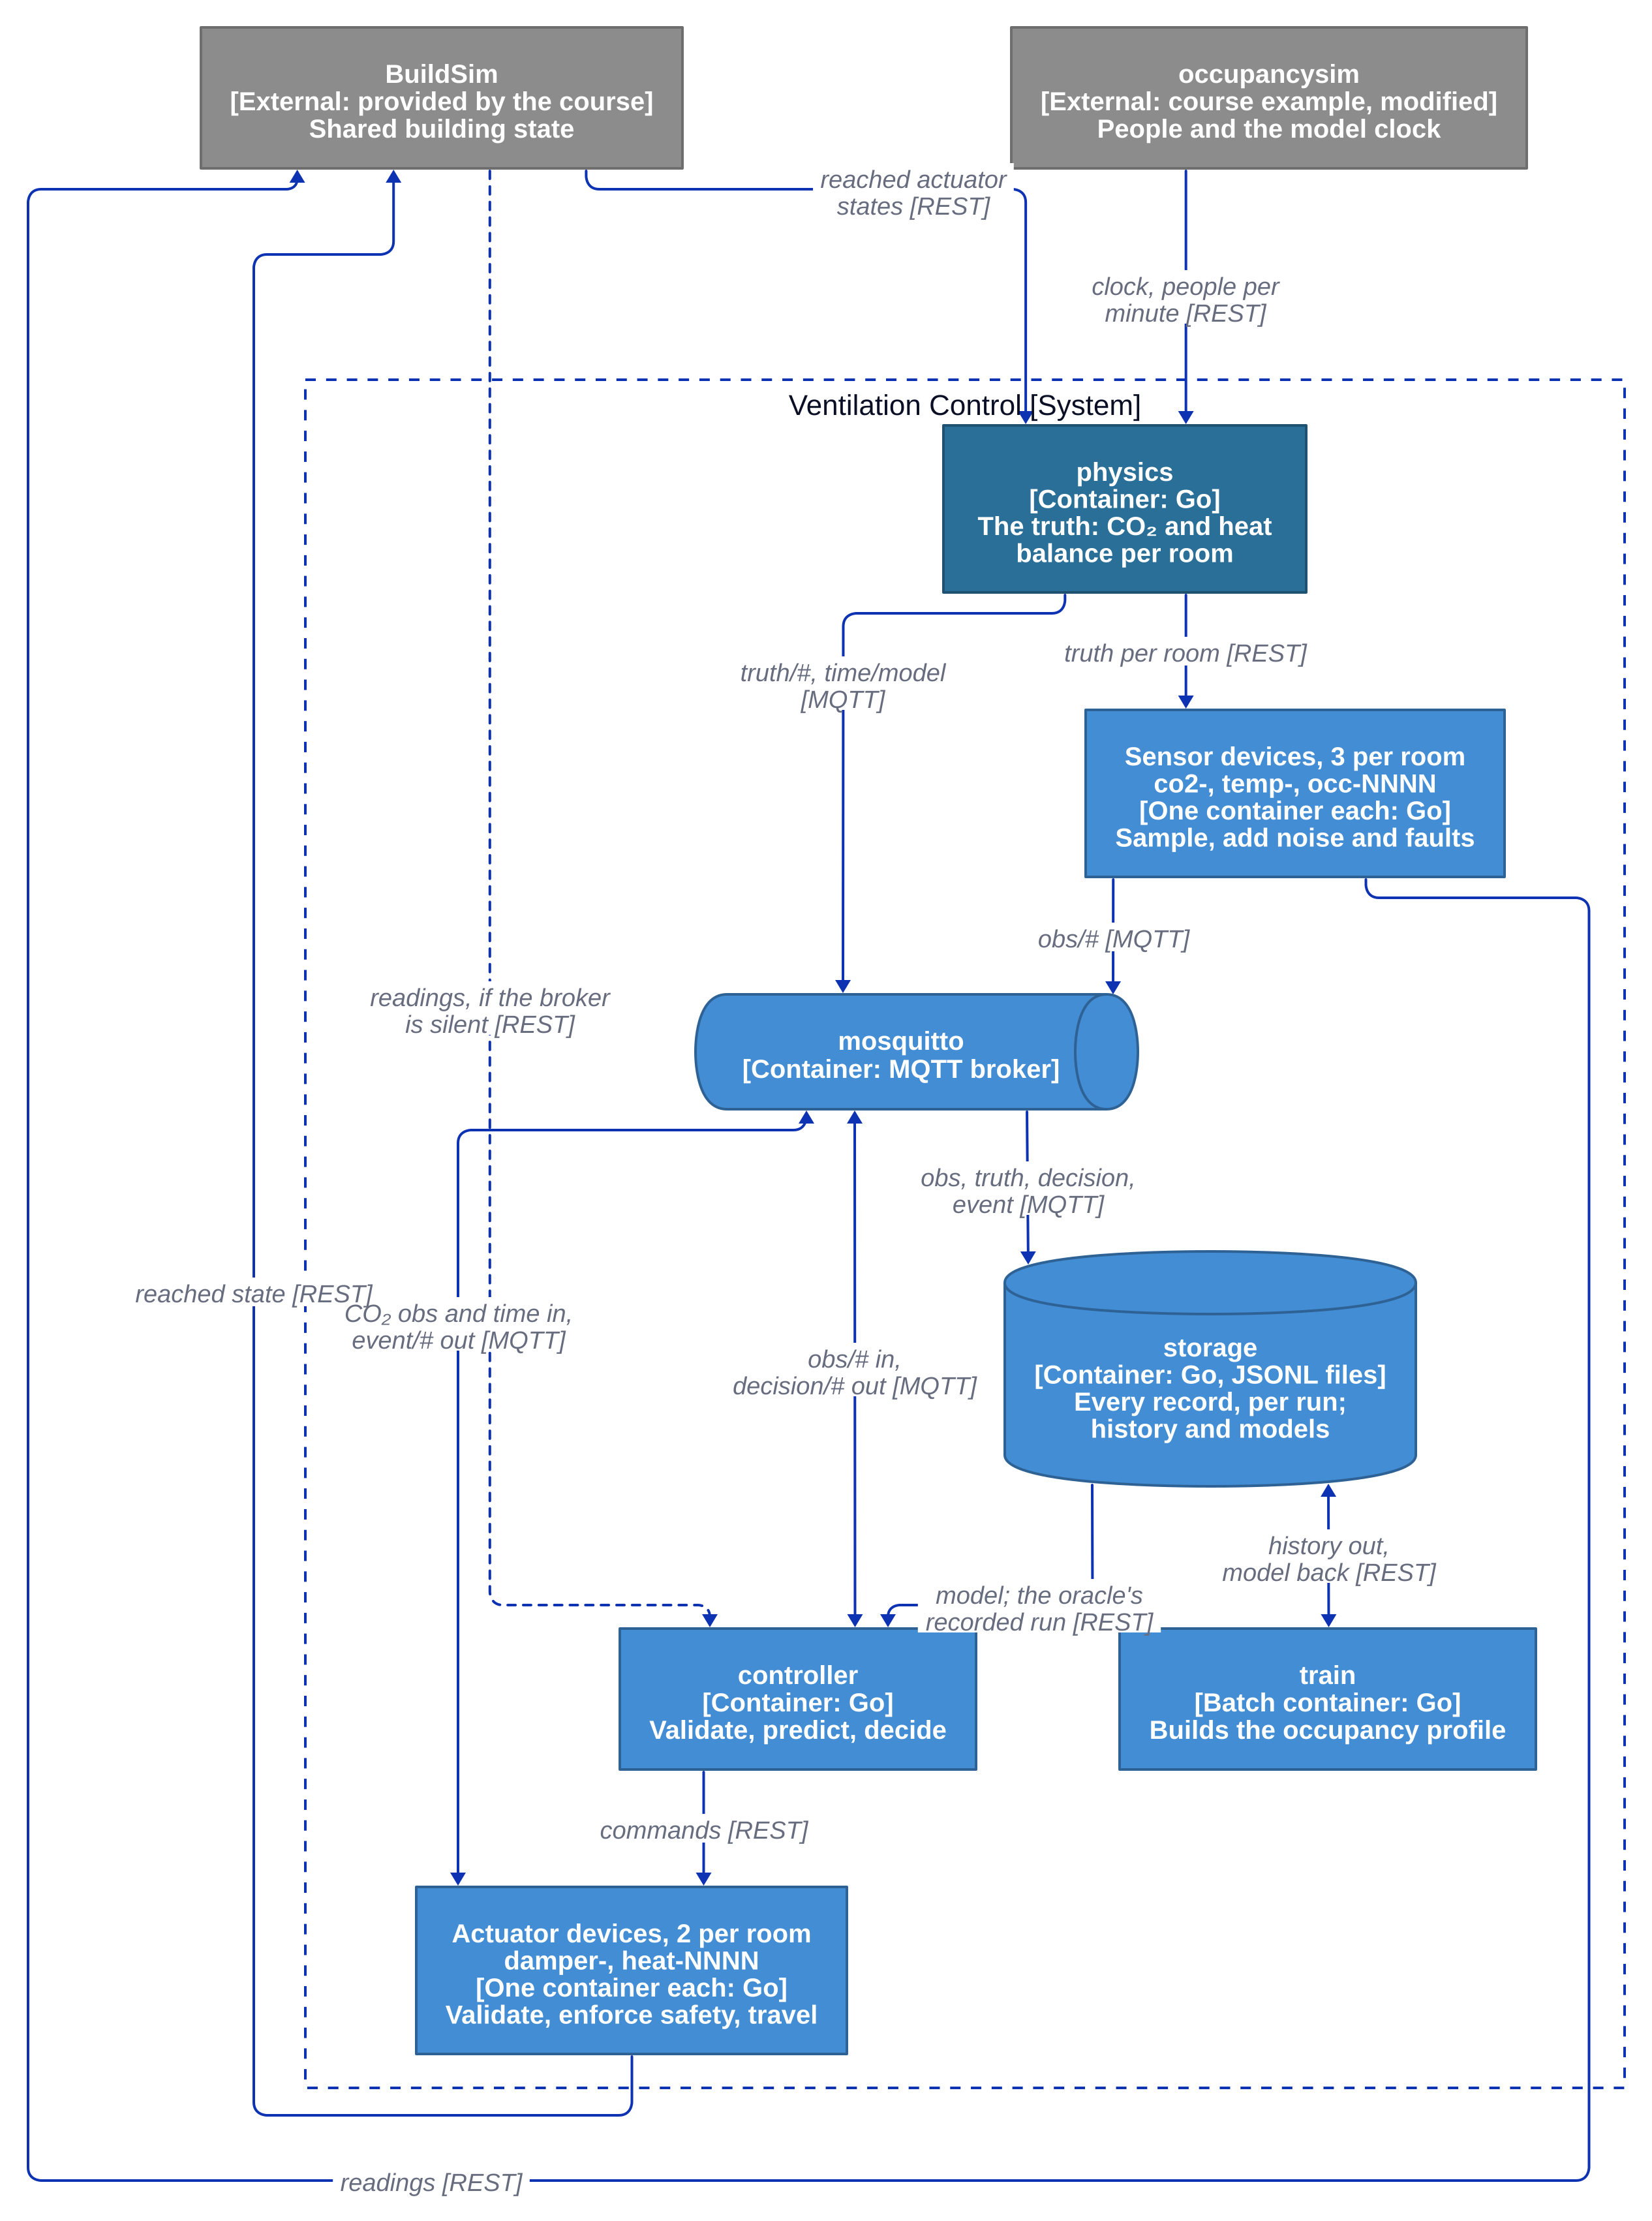
\includegraphics[height=0.78\textheight]{figures/container.png}
\caption{Containers, view 1: the control loop and the data path. One box is one
compose service, except the two device boxes, which are 150 and 100 containers.
The dashed arrow is the controller's fallback when the broker is silent; the
damper has the same fallback for its \COtwo{} reading.}
\label{fig:container}
\end{figure}

\begin{figure}[H]
\centering
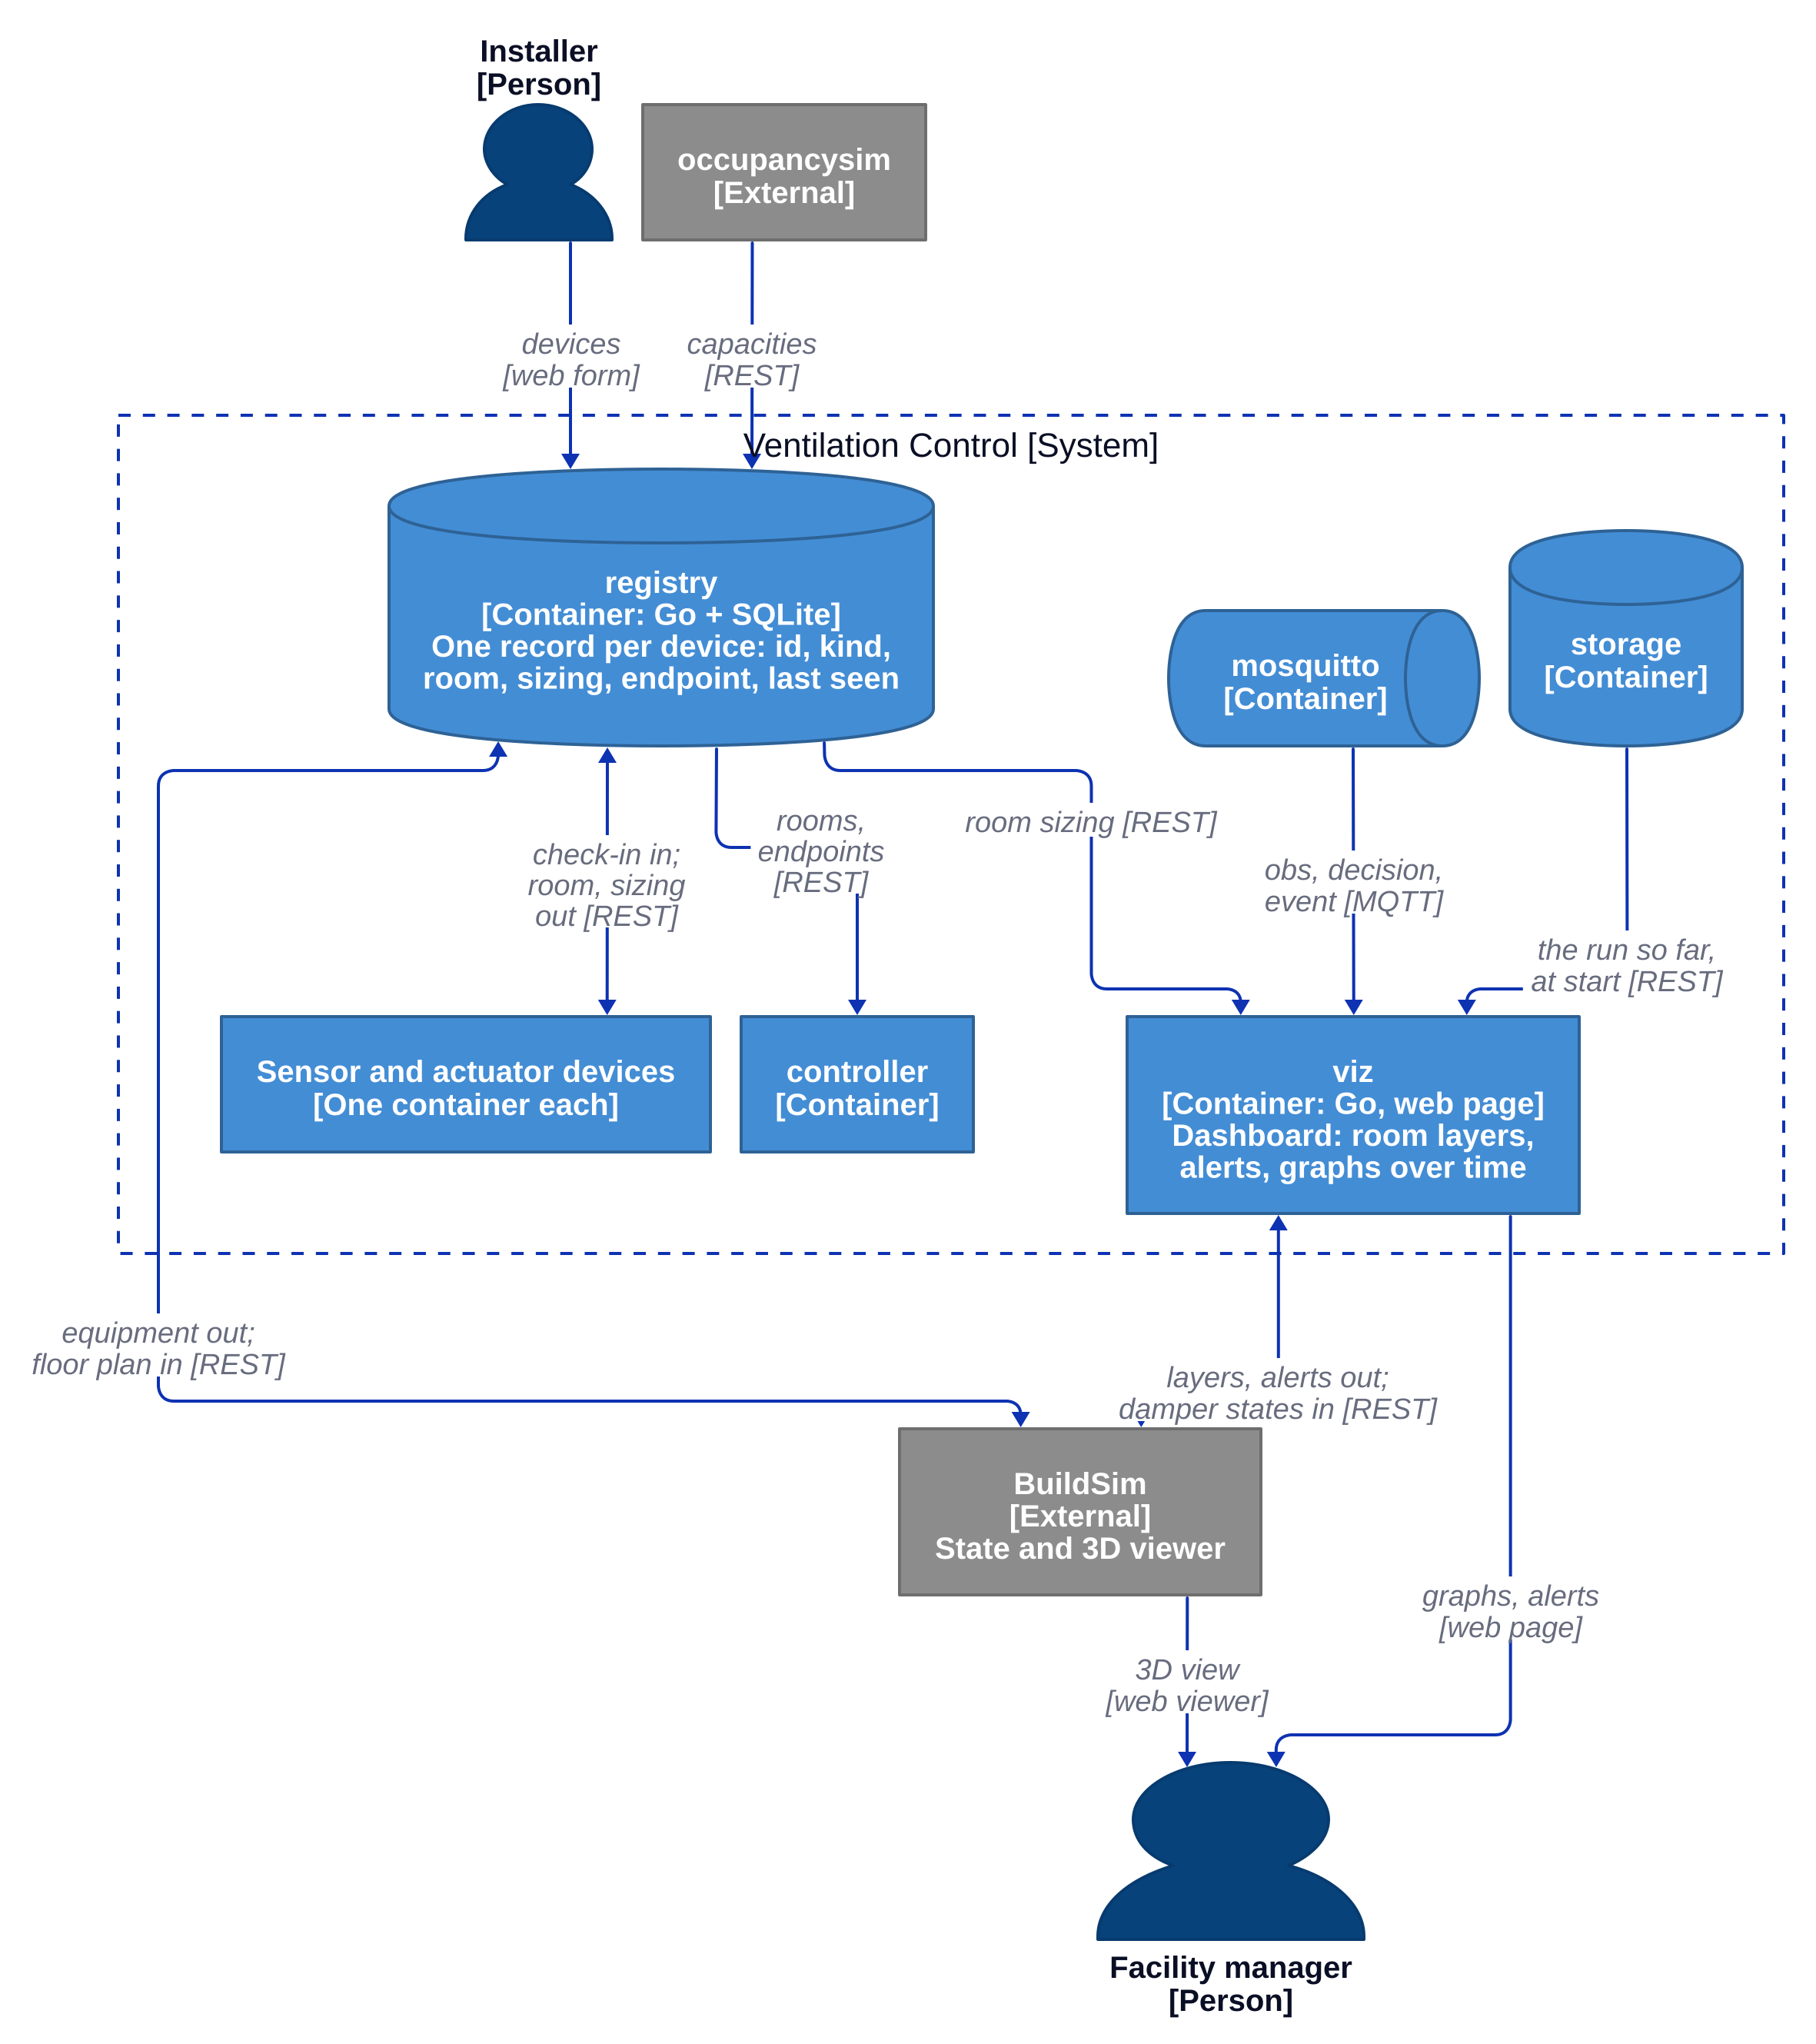
\includegraphics[width=0.74\linewidth]{figures/container-support.png}
\caption{Containers, view 2: commissioning (the registry) and the dashboard
(viz). The devices, the controller, the broker and storage are the same
containers as in Figure~\ref{fig:container}.}
\label{fig:container-support}
\end{figure}

\textbf{The loop.} physics computes each room's true \COtwo{} and temperature
from who is in the room (occupancysim) and from what the room's damper and
radiator valve have reached (read from BuildSim). Each sensor device samples
its own room's truth, adds noise, and reports the reading twice: to BuildSim,
which is the shared state the viewer shows, and to the broker, for everyone who
acts on it. The controller turns readings into commands and sends each command
to the actuator device it is meant for. The actuator validates it, applies the
safety limits, travels towards the target and writes the state it has reached
to BuildSim, where physics reads it. That last step closes the loop.

\textbf{The truth boundary.} Only three things know the true state of a room:
occupancysim, physics, and the sensor devices that sample it. The true state is
published on \code{truth/\#} for the evaluation, and the broker's access list
lets only storage read that topic. Storage in turn refuses to serve the truth
of the run that is in progress. The controller, the actuators and the dashboard
see sensor readings and nothing else. One part of the boundary is a convention
only: the controller shares the compose network with physics and could call its
truth API, although it has no code that does (Section 13).

\textbf{Why each container is its own process.} A network boundary is
justified when a part must be started, stopped, restarted or replaced on its
own. The right-hand column says what would be lost by merging.

\begin{longtable}[]{@{}L{0.14\linewidth}L{0.14\linewidth}L{0.30\linewidth}L{0.32\linewidth}@{}}
\toprule
\textbf{Compose service} & \textbf{Code} & \textbf{Its one job} & \textbf{Why a process of its own} \\
\midrule
\endhead
\code{physics} & \code{cmd/physics} & Compute every room's true state, one
model minute at a time & It is the building. Nothing on the control side may
share memory with it, or the truth leaks \\
\code{co2-NNNN}, \code{temp-NNNN}, \code{occ-NNNN} (150) & \code{cmd/sensor} &
Sample one room, add noise and faults, report & One device, one process, as in
a real installation: a dead sensor silences one room, and a fault is injected
into one device (FR-2, FR-7) \\
\code{damper-NNNN}, \code{heat-NNNN} (100) & \code{cmd/actuator} & Validate
commands, enforce the safety limits, travel, report & The override and the
fallback must work with the controller dead (FR-6, NFR-6) \\
\code{mosquitto} & \code{deploy/ mosquitto} & Carry observations, truth,
decisions, events and the model time & Decouples one publisher from four
consumers; enforces who may read the truth \\
\code{controller} & \code{cmd/controller} & Decide airflow and setpoint per
room & The part most likely to be wrong or replaced; the policy is swapped by
restarting it alone (FR-9) \\
\code{storage} & \code{cmd/storage} & Record every message per run; serve
history and models & Processes may share no files, so the files need one owner
with an API \\
\code{train} & \code{cmd/train} & Build the occupancy profile from stored
readings & Batch work, off the control path; run on demand \\
\code{registry} & \code{cmd/registry} & Know which device is installed where &
Outlives BuildSim restarts; devices and the controller find each other through
it \\
\code{viz} & \code{cmd/viz} & Show the building now and over time & A crashed
dashboard must not stop control \\
\bottomrule
\end{longtable}

The device containers are generated from the installation list:
\code{cmd/gendevices} writes \code{compose.devices.yaml} from
\code{deploy/devices.csv}. \code{cmd/install} and \code{cmd/evaluate} are tools
run by a person, not services.

\textbf{Communication patterns.} Three are used, each where it fits.
\emph{Publish/subscribe} (MQTT, QoS~1) carries the observations, because four
independent consumers need each reading: the controller, the damper's override,
storage and the dashboard. \emph{Request/response} (REST) carries commands,
because the controller needs to know at once whether a command was accepted,
clamped or refused; commands carry an id and a time to live, so a retry is
safe. \emph{Shared state} (BuildSim) is the fallback for both directions: when
the broker is silent, the controller and the dampers poll the readings there.
The model time is one retained MQTT message that physics refreshes every tick,
the way a building network distributes time to its devices.

\subsection{4.3 Component diagram (C4 Level 3): the controller}

\begin{figure}[H]
\centering
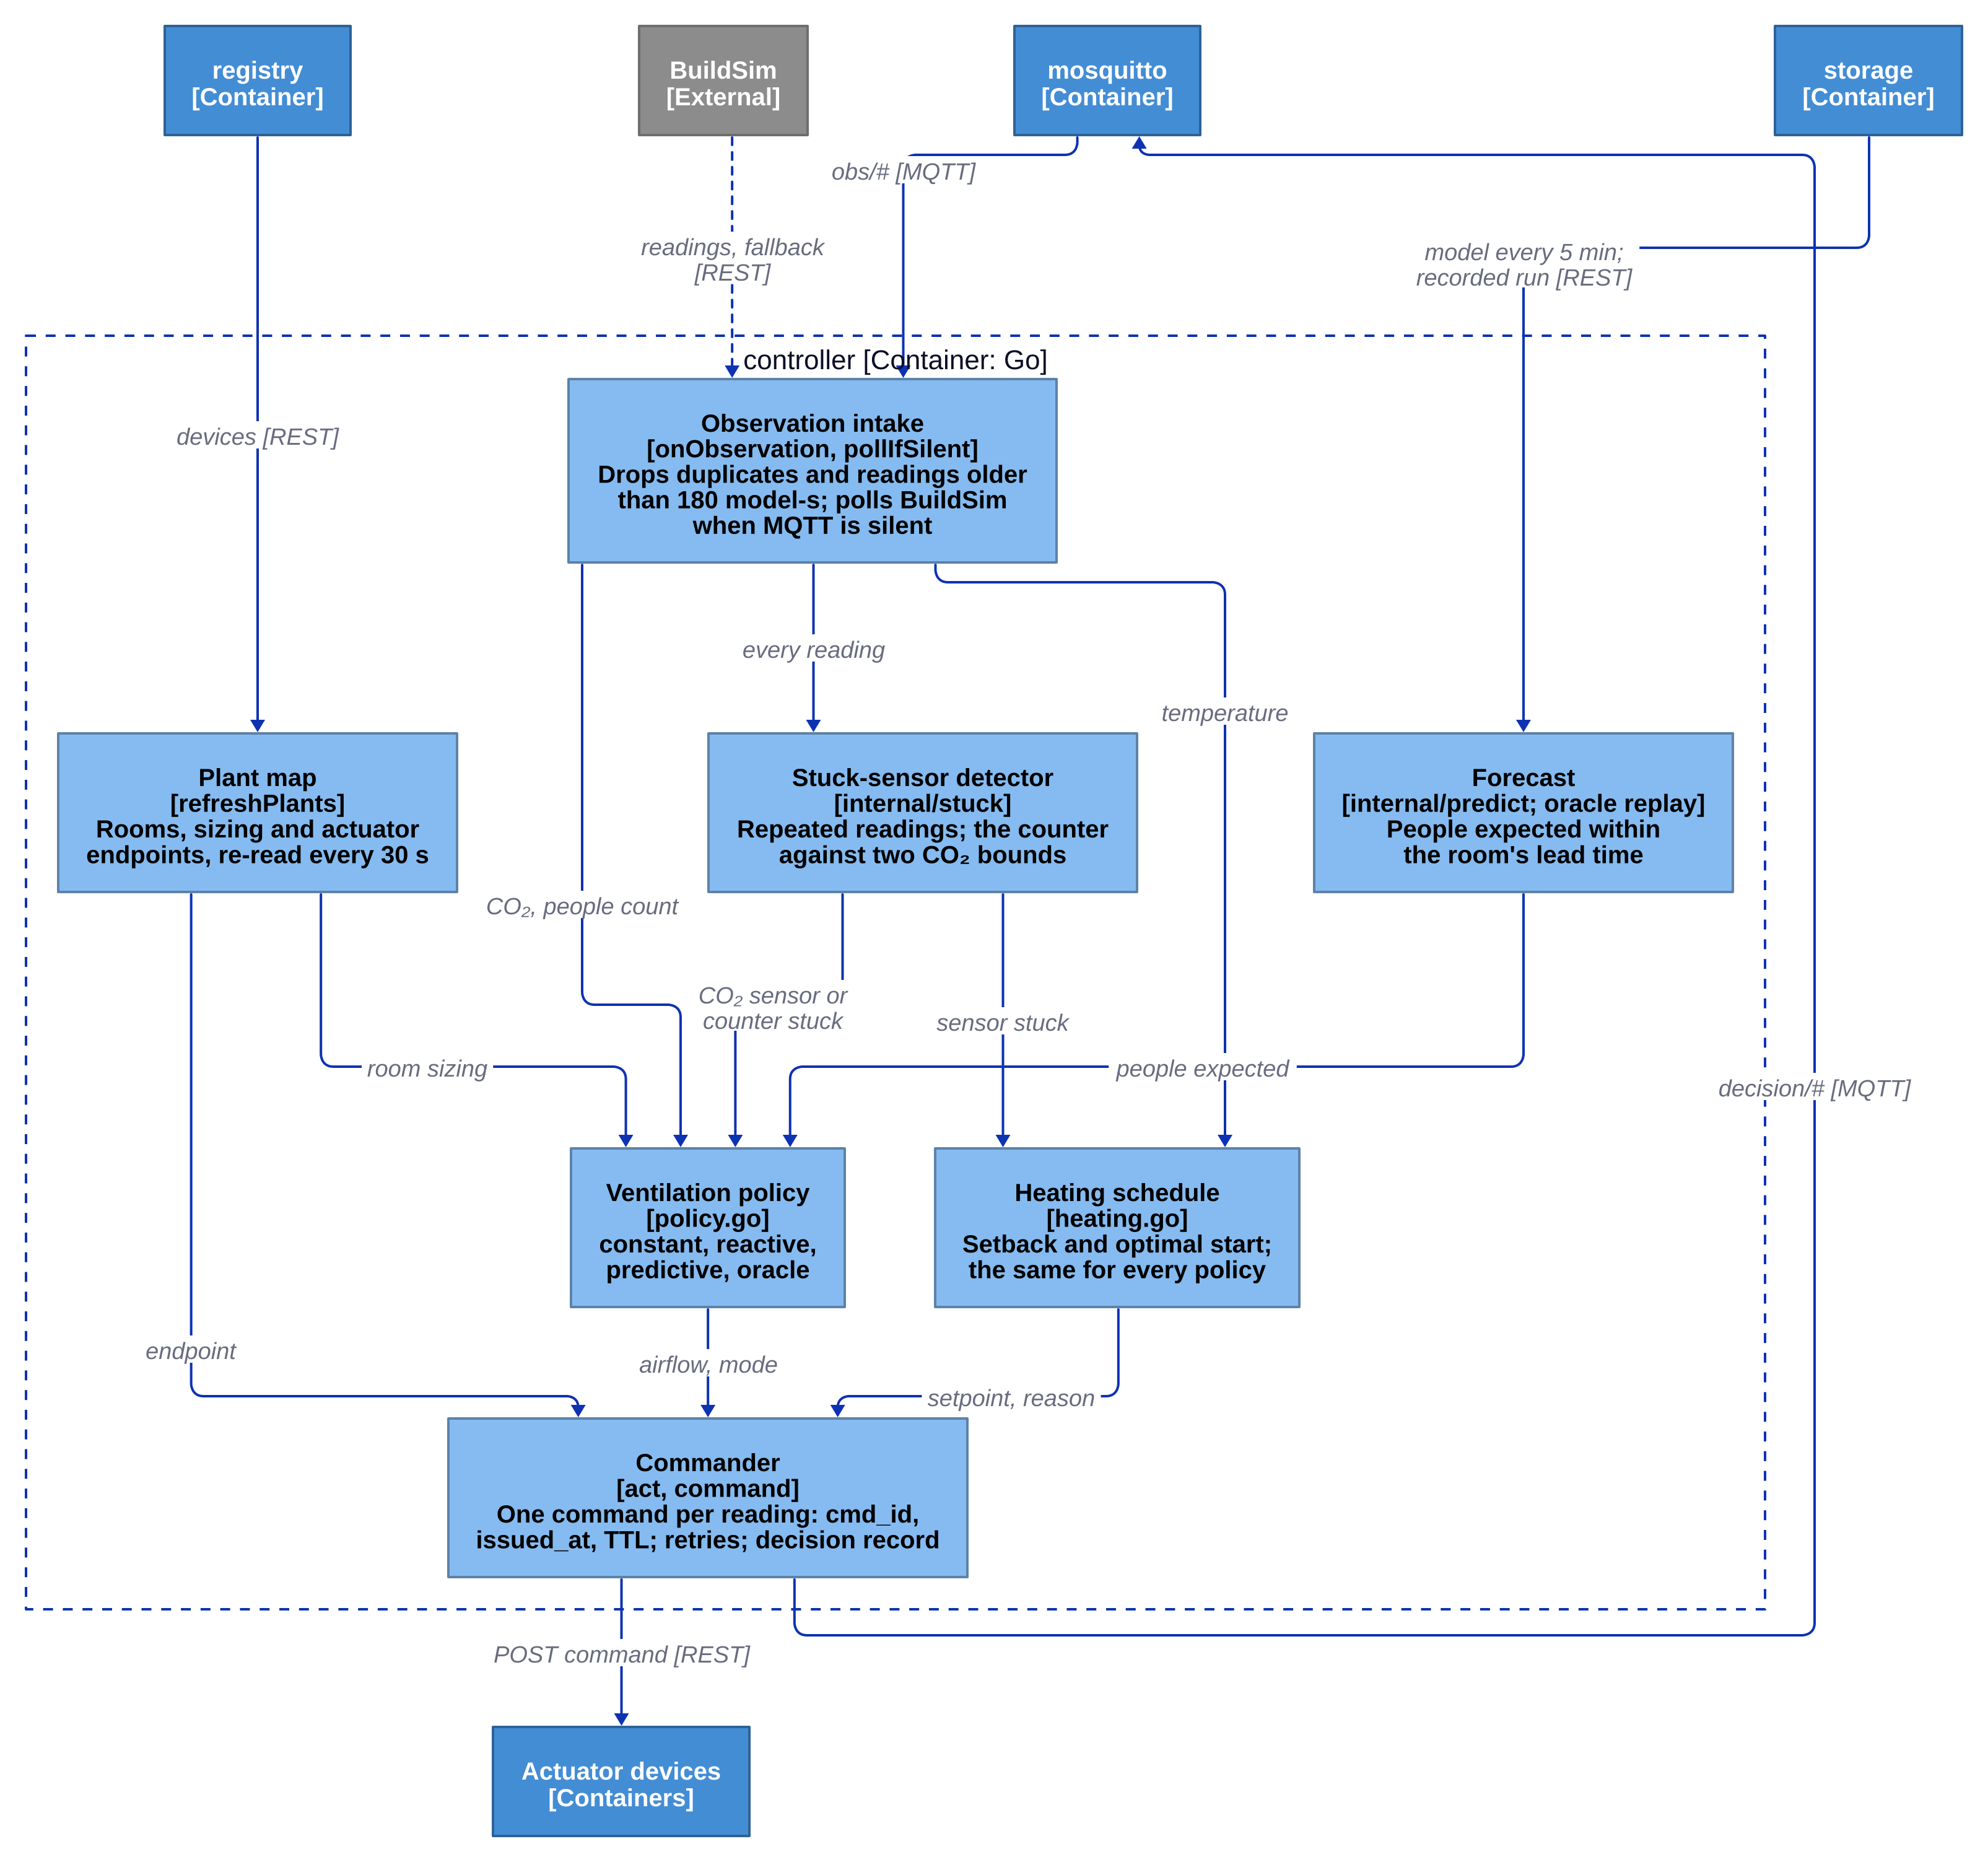
\includegraphics[width=0.92\linewidth]{figures/component.png}
\caption{Components of the controller. Each is a Go file or package in
\code{cmd/controller} and \code{internal/}.}
\label{fig:component}
\end{figure}

The controller makes one decision per reading. A \COtwo{} reading leads to an
airflow command for that room's damper, a temperature reading to a setpoint
command for its radiator valve, and a people count is remembered for the next
airflow decision. The \emph{observation intake} drops duplicates and readings
older than 180~s. The \emph{stuck-sensor detector} sees every reading and tells
the policy when a sensor's value can no longer be believed. The \emph{forecast}
answers one question, how many people to expect within the room's lead time,
either from the trained profile or, for the oracle, from the recorded truth of
an earlier run of the same dates. The \emph{ventilation policy} and the
\emph{heating schedule} are pure functions of those inputs. The
\emph{commander} sends the command, retries with the same id, and publishes the
decision record with what the actuator answered.

The split follows what changes independently. The four policies differ only in
the ventilation policy component, which is what makes the comparison in Section
11 fair. The forecast keeps the last model it loaded, so storage can be down
without the policy noticing.

\subsection{4.4 Design decisions and alternatives}

\begin{longtable}[]{@{}L{0.05\linewidth}L{0.24\linewidth}L{0.24\linewidth}L{0.07\linewidth}L{0.28\linewidth}@{}}
\toprule
\textbf{\#} & \textbf{Chosen} & \textbf{Alternatives rejected} & \textbf{Serves} & \textbf{Why, and the trade-off accepted} \\
\midrule
\endhead
D-1 & \textbf{Time.} Physics advances by whole model minutes from
occupancysim's per-minute record; every observation carries model time &
Each service keeps its own wall-clock × factor; physics samples BuildSim's
occupancy on its own tick & FR-1, NFR-7 & The second alternative is what we
built first: two runs of one day then disagreed in 0.3~\% of samples.
Trade-off: physics depends on an endpoint we added to occupancysim \\
D-2 & \textbf{Sensors.} One container per sensor device, sampling its room
from a truth API on physics & Physics writes noisy values to BuildSim itself;
one gateway per sensor kind & FR-2, FR-7 & The first breaks the one-process
rule and puts truth and observation in one process. The second, built first,
silences a whole kind when it crashes. Trade-off: 150 containers \\
D-3 & \textbf{Transport.} Sensors write to BuildSim and publish to MQTT;
consumers subscribe; BuildSim polling is the fallback & Everyone polls
BuildSim; a separate collector that polls and republishes & NFR-5, NFR-6 &
Four consumers need each reading. A collector adds a hop for data the sensor
already has. Trade-off: a broker to run, and two writes per reading that are
not atomic \\
D-4 & \textbf{Storage.} A storage service owns JSONL files per run and serves
them over HTTP & Files shared between logger, trainer and controller;
TimescaleDB & FR-8, NFR-7 & Shared files break a course rule. A database
server is hard to justify at 50 rooms. Trade-off: a history query reads the
whole run \\
D-5 & \textbf{Autonomy.} Validation, forecast and policy in one controller;
training as a batch job & The predictor as its own service & FR-3, FR-4 & No
network hop on the control path, and nothing else needs the forecast.
Trade-off: the parts cannot be restarted separately \\
D-6 & \textbf{Safety.} Enforced in the actuator: range, rate, TTL, flow
floors, \COtwo{} override & Inside the controller, after the policy; a
separate safety process & FR-5, FR-6, NFR-6 & It must survive a dead or wrong
controller. Trade-off: the damper needs the room's sizing and the \COtwo{}
stream, so it is no longer a plain device \\
D-7 & \textbf{Baselines.} One policy interface, four implementations; the
oracle replays the recorded truth of an earlier run of the same dates & An
oracle that reads occupancysim's plans & FR-9, NFR-7 & The oracle then uses
the same forecast interface as the predictor and never touches live truth.
Trade-off: it needs two runs of a day to be identical, which needed D-1 \\
D-8 & \textbf{Dashboard.} A viz process: layers and alerts in the BuildSim
viewer, and its own page of graphs & The viewer alone; Grafana over storage &
FR-10 & The viewer has no history. Grafana would need an index on our files
first. Trade-off: the graphs' history is a second copy, in viz's memory \\
D-9 & \textbf{Actuators.} One container per actuator device & One container
per kind for all rooms; one for everything & FR-5, NFR-6 & A failed damper
affects one room. Trade-off: 100 containers \\
D-10 & \textbf{Commissioning.} A registry with its own database; a device
learns its room at check-in & Device lists in configuration; registering
straight in BuildSim & FR-11 & BuildSim forgets everything on restart, and
configuration means nobody installs anything. Trade-off: one more service on
the start-up path, and devices do not authenticate \\
D-11 & \textbf{Stuck sensors.} A run of identical readings for \COtwo{} and
temperature; the counter against two \COtwo{} mass-balance bounds that hold
for any airflow & ``Counter unchanged while \COtwo{} moves''; estimating the
head-count from \COtwo{} and airflow & FR-7 & The first blames every healthy
counter when a lecture starts, because \COtwo{} lags the count. The second
needs the damper's true flow at every moment. Trade-off: blind to small
over-counts, and slow (15--75~min) \\
-- & \textbf{Room set.} 50 rooms on one floor, a fixed seeded sample & The
whole building (838 rooms); all of the floor (277) & NFR-5, NFR-8 & One
container per device makes the laptop the limit (Section 11). Trade-off: about
60~\% of the floor's lectures land in rooms we do not simulate \\
\bottomrule
\end{longtable}

Three of these were reversed by evidence, which is why their first versions
appear as rejected alternatives. D-1 and D-7: the oracle was designed on the
assumption that two runs of a day are identical, and the first evaluation
showed they were not. D-2 and D-9: gateways per kind were built first and
replaced by one process per device after the lecturer suggested an installer's device database. D-8: the viewer
alone was the first decision, and it could not answer how a room got to where
it is.
